\documentclass[11pt]{report}
\usepackage{geometry}
\usepackage{multirow}
\usepackage{array}
\usepackage{xcolor, colortbl}
\usepackage{makecell}
\usepackage{tabularray}
\usepackage[export]{adjustbox}
\geometry{top = 50pt, bottom = 50pt, left = 1in, right = 1in }
\usepackage{graphicx}
\usepackage[T1]{fontenc}
\usepackage{fourier}
\usepackage{setspace}
\usepackage[acronym,shortcuts]{glossaries}
\makenoidxglossaries
\usepackage{url}
\usepackage[hidelinks]{hyperref}

\setlength{\tabcolsep}{18pt}
\renewcommand{\arraystretch}{1.5}

%This is used to control splitting of words using hyphen in LaTeX
\tolerance=9999
\emergencystretch=10pt
\hyphenpenalty=10000
\exhyphenpenalty=100

\loadglsentries{Chapters/abbreviations.tex}

%\rhead{
\includegraphics[width=1cm]{Logo/Thws-logo_English.png}}


%%FOR ADDING HEADER %%%
%\pagestyle{fancy}
%\renewcommand{\chaptermark}[1]{\markboth{#1}{#1}}
%\fancyhead{}
%\fancyhead[L]{\chaptername\ \thechapter\ --\ \leftmark}
%\fancyhead[R]{
\includegraphics[height=0.75cm]{Logo/bosch_logo.png}}
%%\fancypagestyle{plain} %-->To show header on the starting of all Chapters
%\pagestyle{plain}
%\fancyfoot{}
\pgfplotsset{compat=1.18}
\begin{document}

\pagenumbering{Roman}
\begin{titlepage}
    \par
    
\includegraphics[width=0.3\textwidth, valign=M]{Logo/bosch_logo.png}
    \hfill
    
\includegraphics[width=0.3\textwidth,valign=M]{Logo/Thws-logo_English.png}
    \par
    \vspace{3cm}
    \begin{center}
         \textbf{\Huge Bachelor Thesis}
         \vspace{5pt}
         \\
         for the bachelors degree program in Mechatronics
         \vspace{2.5cm}
         \\
         \textbf{\Huge Development of a Continuous Integration (CI) framework for OptiSlang workflows}
         \vspace{2cm}
         \\
         In co-operation with
         \vspace{5pt}
         \\
         Robert Bosch GmbH
         \vspace{2cm}
         \\
         Author : Sathvick Bindinganavale Srinath\\
         Matriculation Number : 4020025
         \vspace{1cm}\\
         Supervisor : Mr. André Haeitmann Dutra \\
         1\textsuperscript{st} Examiner : \\
         2\textsuperscript{nd} Examiner :
         \vspace{1cm} \\
         Submission Date : 
    \end{center}
\end{titlepage}
\vspace*{3cm}
\begin{center}
    \textbf{\Huge DECLARATION}
\end{center}
\vspace{2cm}
\begin{onehalfspace}
    I, Sathvick Bindinganavale Srinath, declare that the work in this thesis, \textbf{"Development of a \acrlong{ci} Framework for OptiSlang Workflows"} was carried out in accordance
with the regulations of the Technical University of Applied Sciences Würzburg-Schweinfurt. I have clearly marked and acknowledged all direct quotations and all information obtained from other sources. I have not used any
other sources or resources than those indicated. I have not submitted this thesis to any other examination board.
\end{onehalfspace}

\vspace{1cm}

\vspace*{4em}\noindent
\hfill%
\begin{tabular}[t]{c}
  Ludwigsburg, 05.10.2024\\\rule{10em}{0.4pt}\\ Place, Date
\end{tabular}%
\hfill%
\begin{tabular}[t]{c}
%!Add image of signature here

\includegraphics[width=0.35\textwidth]{Images/signature.pdf}\\\rule{10em}{0.4pt}\\ Signature
\end{tabular}%
\hfill\strut
\tableofcontents
\listoffigures
\addcontentsline{toc}{chapter}{List of Figures}
\lstlistoflistings
%\addcontentsline{toc}{chapter}{List of Tables}
\addcontentsline{toc}{chapter}{Abbreviations}
{\Large\printnoidxglossary[type=\acronymtype, style=dotlist, title=Abbreviations, nonumberlist]} %nonumberlist prevents adding page number to the glossary.
%\chapter*{Abstract}
%\textbf{Better to write this after finishing all the chapters}\\
%Hello, this is an abstract \\
%(Write something about CI as an introduction here)\\
%Sections to be written: (Please do not write in future tense)\\
%- Objective\\
%- Research Methods\\
%- Results\\
%- Conclusion\\
%- (Optional) Keywords
\begin{abstract}
System developers at Bosch create modules in MATLAB and Python to address specific use cases. These modules are integrated into Optislang, a software tool used 
for optimization analysis. For every new feature in the modules, developers must generate a new version and test it locally, a process that is both time-consuming 
and error-prone. This thesis proposes a solution to automate the testing of these modules. The modules are executed using a Python-based framework, which is 
integrated into a \acrfull{ci} pipeline on GitHub. This pipeline is triggered whenever a new commit is pushed to the repository, running the 
tests and providing feedback to the developers. By implementing this solution, developers receive immediate feedback and can focus more on developing new 
features.
\end{abstract}
\addcontentsline{toc}{chapter}{Abstract}
\cleardoublepage\pagenumbering{arabic}
\begin{spacing}{1.17}

\chapter{Introduction}
\section{Overview}
This thesis explains about the creation and development of a framework for Optislang workflows. The workflow mostly contains modules created using Python and
MATLAB.


\section{Objective}
The objective of this thesis are as follows:
\begin{itemize}
    \item Develop a method to create a standalone version of MATLAB and Python based modules in Optislang for integration testing (only code based, without using 
    \acrshort{gui}).
    \item Implement workflows in batch mode.
    \item Create a framework in Python to create modules and workflows.
    \item Establish a strategy to for automated integration testing in Github for modules based on Python and MATLAB. 
\end{itemize}

\section{Outline}
\begin{itemize}
    \item   In Chapter 2, we are going to discuss about the \acrshort{moo} project, its role in the company and the modules created in Python and Optislang.
    \item   In Chapter 3, we understand the creation of a framework to create standalone modules and workflows in Python.
    \item   In Chapter 4, we will look into the automated integration testing in Github.
    \item   In Chapter 5, we will discuss the results and evaluate the impact of the solution.
    \item   Finally, Chapter 6 provides us the summary of the work, highlighting the achievements and feedback for development in potential areas.
\end{itemize}
\chapter{\acrlong{moo}}

%%%%%%%%%%%%%%%%%   SECTION : INTRODUCTION   %%%%%%%%%%%%%%%%%%%%%%%%%%%%%%
\section{Introduction} \label{what is moo}
In today's increasingly complex world, decision-makers often face the challenge of optimizing several conflicting objectives simultaneously. \acrfull{moo} 
is an optimization that deals with such problems, where multiple objective functions are optimized simultaneously. To understand \acrshort{moo} better, 
let us consider an example.

\paragraph{Example:}
Let us consider an example of a car manufacturer. The car consists of many components like engine, body, wheels, etc which can be
tweaked. In our case, the manufacturer wants to optimize the car for two objectives: lower manufacturing cost of the car and lower carbon emissions. With 
considering the input parameters and the objectives, we get many solutions as shown in Figure \ref{moo}

\begin{figure}[!h]
	\begin{center}
		\input{../Python/plots/moo_plot.tex}
	\end{center}
    \caption{Example of \acrshort{moo}}
    \label{moo}
\end{figure}
In an \acrshort{moo} problem, there typically is no single best solution. Rather, the \textit{goal} is to identify a set of solutions that are optimal in terms 
of all objectives. In Figure \ref{moo}, the best solutions for the given objectives is indicated in orange known as pareto optimal solutions. A solution is said 
to be pareto optimal if no other solution can improve on any of the objectives without worsening at least one of the other objectives.
%The solutions which are not Pareto optimal are not considered as they are dominated by the Pareto optimal solutions. 

\section{Difference between \acrshort{moo} and \acrshort{soo}}
Optimization problems, whether single-objective or multi-objective, have the same goal: to find the best solution(s) to a given problem. However, the approach
to solving these problems is different. 

In \acrfull{soo}, the goal is to optimize a single objective function, which can either be maximized or minimized. The  problem is simpler to define and solve
because it involves only one objective. To calculate \acrshort{soo}, we can use methods like gradient descent, linear programming, etc.

\begin{figure}[!h]
    \centering
    \input{../Python/plots/soo_plot.tex}
    \caption{Example of \acrshort{soo}}
    \label{soo}
\end{figure}

In Figure \ref{soo}, we have considered the same example given in section \ref{what is moo}. But, here, we are considering only one objective, which is to
minimize the manufacturing cost. The best solution is indicated in orange.
\vspace{15pt}

In \acrshort{moo}, the optimization involves two or more objective functions simultaneously. The problem is more complex because the objectives are often
conflicting. Unlike \acrshort{soo}, where we have a single best solution, in \acrshort{moo}, we have pareto optimal solutions.
To calculate \acrshort{moo}, we can use methods like pareto optimization, scalarization method, weighted sum method, $\epsilon$-constraint method, etc.


While \acrshort{soo} focuses on finding the best solution according to a single criterion, \acrshort{moo} addresses the more complex task of balancing multiple, 
often conflicting objectives. The choice between \acrshort{soo} and \acrshort{moo} depends on the nature of the problem at hand and the goals of the decision-maker. 
Understanding the differences between these approaches is crucial for selecting the appropriate optimization technique and achieving the desired outcomes.

%%%%%%%%%%%%%%%   SECTION : OPTISLANG  %%%%%%%%%%%%%%%%%%%%%%%%%%%%%%%%
\section{Optislang}
\paragraph{}

To calculate \acrshort{moo}, we need a software platform that can handle the complexity of the problem. Ansys Optislang \cite{optislang} is such a software 
platform, which is used for design exploration, \acrfull{cae} based sensitivity analysis and optimization in conjunction with any product development tool. 
It is a Process Integration and Design Optimization tool or in short, a \acrshort{pido} tool. Process Integration refers to automate and orchestrate manual 
simulation processes and to realize complex workflows. Design Optimization aims for better understanding of your design, optimizing the product, identify an 
improved design which has the desired qualities and resulting in a best design by reliability analysis and statistical analysis.  


Optislang uses several solvers to look into aspects like mechanical, technical, mathematical and any other problems. This is easier in Optislang as it provides
integration to create toolchains of many external programs like ANSYS, MATLAB, Excel, Python, CATIA and many more.


Our department utilizes Optislang for solving \acrshort{moo} problems, as it includes algorithms specifically designed for \acrshort{moo}.
%# Try to explain about the parametric system, sensitivity analysis, MOP, ...
%%%%%%%%%%%%%%%%%   SECTION : MODULES AND WORKFLOWS   %%%%%%%%%%%%%%%%%%%%%%%%%%%%%%
\section{Modules and Workflows}
\subsection{Modules}
Modules are created by the system developers. Modules include a simulation model as a calculation with defined interfaces for coupling with other modules. 
These modules are either defined in MATLAB or Python. Each module is designed to tackle/improve a specific issue. To document and collaborate with other
system developers, each module is versioned and stored in a specific manner in a repository in GitHub Enterprise.

\begin{figure}[!h]
    \centering
    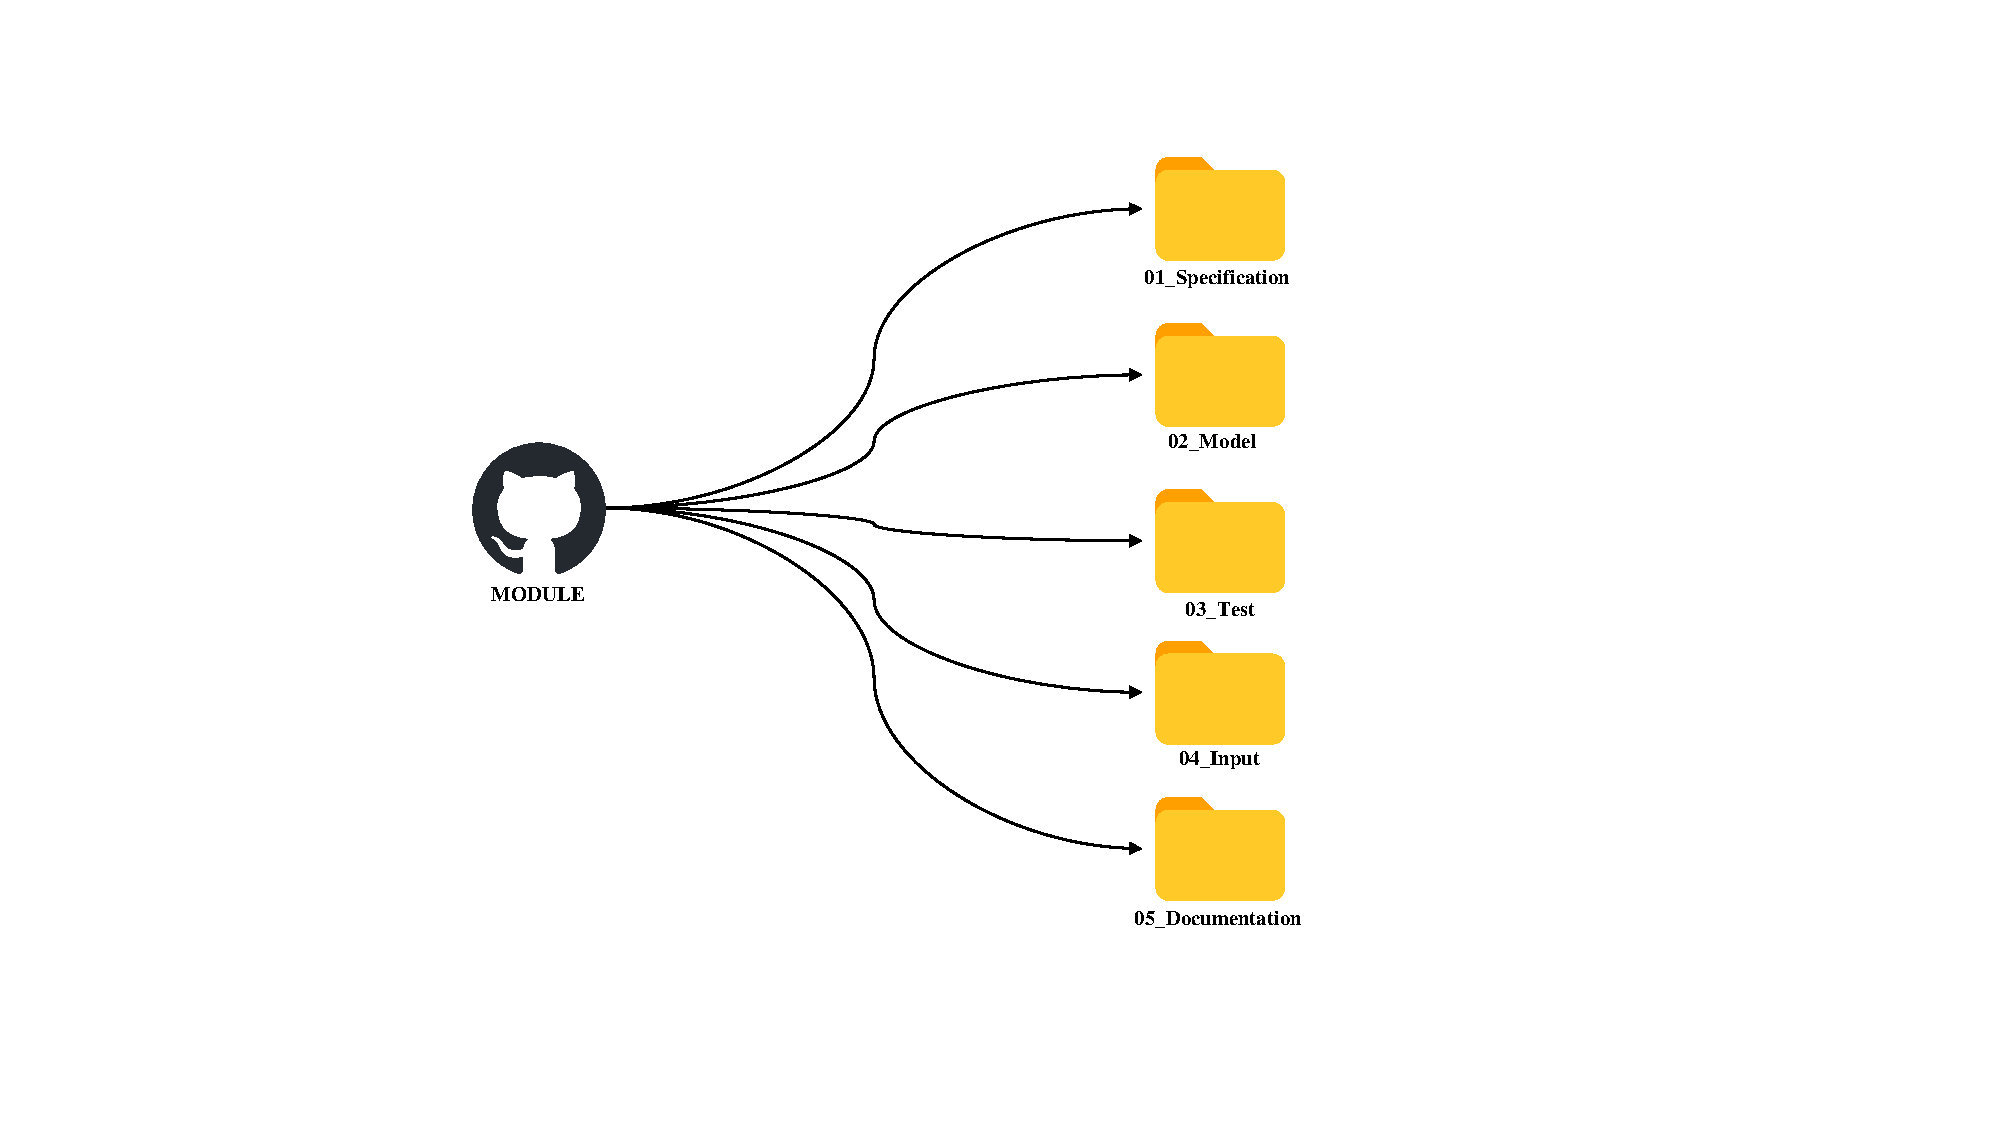
\includegraphics[width=1.2\textwidth]{Images/github_folder_structure.pdf}
    \caption{Example of a module's GitHub repository structure}
    \label{github_arrhenius}
\end{figure}

Figure \ref{github_arrhenius} shows us an example of how each module is maintained in our GitHub organization.
\begin{itemize}
    \item \verb|01_Specification| has all the requirements for the module to run.
    \item \verb|02_Model| contains all parts to run the model. This can also be used as a playground for the development of a model.
    \item \verb|03_Test| contains all the unit tests for the module. This is to ensure that the module is working as expected.
    \item \verb|04_Input| carries all the initial parameters or functions to be defined at the start of a module.
    \item \verb|05_Documentation|contains documents explaining functioning and usage of the module.
\end{itemize}
%\begin{table}[!h]
%    \begin{tabular}{|>{\centering\arraybackslash}p{2cm}|>{\centering\arraybackslash}p{12cm}|}
%        \hline
%        Name of the module & \multirow{2}{*}{\centering Use Case}\\
%        \hline
%        Pv Calculator & Simulation of FET losses as input for the FET's temperature estimation as base for a first reliability prognosis\\
%    \end{tabular}
%\end{table}
\subsection{Workflows}
Our department develop automatized workflows for power electronics products considering functional loads to reliability indications. Workflows are a sequence
of modules designed for a fast calculation performance characteristic like temperature or reliability indication. To develop a workflow, Optislang is used.


Every architectural workflow has a GitHub repository that is maintained in a similar way to how modules are being maintained.

\begin{figure}[!h]
    \centering
    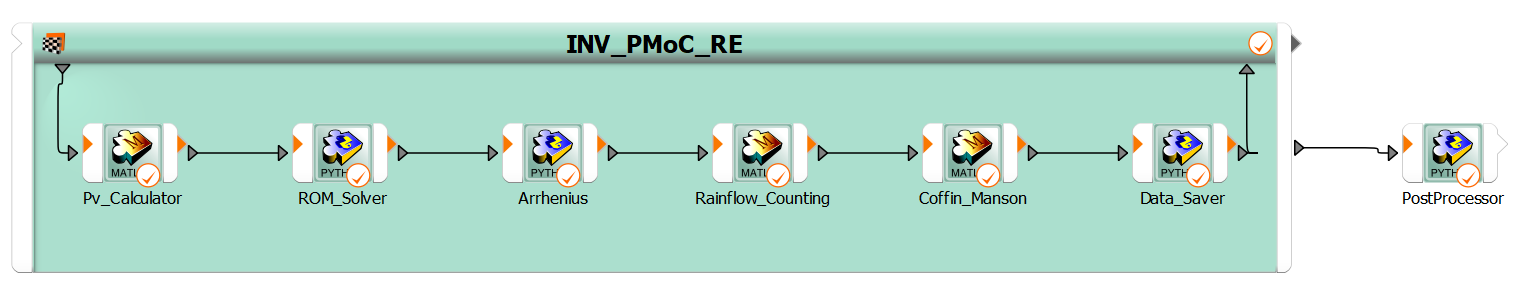
\includegraphics[width=\textwidth]{Images/workflow_example.png}
    \caption{Example of a workflow in Optislang}
    \label{workflow_example}
\end{figure}

%%%%%%%%%%%%%%%%%   SECTION : CURRENT PROBLEM   %%%%%%%%%%%%%%%%%%%%%%%%%%%%%%
\section{Current Problem} \label{current problem}
lorem ipsum dolor sit amet, consectetur adipiscing elit. Donec auctor, nunc nec lorem ipsum dolor sit amet, consectetur adipiscing elit. Donec auctor, nunc
nec lorem ipsum dolor sit amet, consectetur adipiscing elit. Donec auctor, nunc nec lorem ipsum dolor sit amet, consectetur adipiscing elit. Donec auctor, nunc
nec lorem ipsum dolor sit amet, consectetur adipiscing elit. Donec auctor, nunc nec lorem ipsum dolor sit amet, consectetur adipiscing elit. Donec auctor, nunc
nec lorem ipsum dolor sit amet, consectetur adipiscing elit. Donec auctor, nunc nec lorem ipsum dolor sit amet, consectetur adipiscing elit. Donec auctor, nunc
nec lorem ipsum dolor sit amet, consectetur adipiscing elit. Donec auctor, nunc nec lorem ipsum dolor sit amet, consectetur adipiscing elit. Donec auctor, nunc
lorem ipsum dolor sit amet, consectetur adipiscing elit. Donec auctor, nunc nec lorem ipsum dolor sit amet, consectetur adipiscing elit. Donec auctor, nunc
nec lorem ipsum dolor sit amet, consectetur adipiscing elit. Donec auctor, nunc nec lorem ipsum dolor sit amet, consectetur adipiscing elit. Donec auctor, nunc

 %#! Explain why it is time consuming to test the module, labour intensive, increase of errors with complexity of the module/workflow
 %#! Explain the lack of standardization of module, difficulty in maintaining the modules effectively
\chapter{Related Work}
\section{\acrlong{ci} in Software Development}
\acrfull{ci} is a software development practice that integrates code changes frequently and tests them automatically to detect issues early in the development 
process. The concept of \acrshort{ci} was popularized by Martin Fowler in the early 2000s, emphasizing the importance of automating the build and test 
process to ensure code stability\cite{fowler2006continuous} . Jenkins\footnote{\url{https://www.jenkins.io/}} and Travis CI\footnote{\url{https://www.travis-ci.com}} 
are two of the most widely adopted CI tools that automate build processes and testing in a wide range of programming environments. These tools have laid the 
groundwork for integrating code quality checks, reducing effort of manual testing.

More recently, GitHub Actions\cite{github_actions} has gained popularity as a \acrshort{ci} tool integrated directly within GitHub repositories, enabling developers to automate 
workflows triggered by events like code pushes or pull requests. Similar to these approaches, the framework developed in this thesis leverages GitHub Actions 
to automate testing of OptiSlang modules, ensuring real-time feedback to developers\cite{8444829}.

\section{Automation in Simulation based Optimization Workflows}
Automation of simulation-based optimization workflows has a significant focus in engineering domains. Industries like automotive, aerospace, and manufacturing
rely heavily on simulation tools like MATLAB and Ansys to optimize designs. These tools are often integrated with optimization algorithms to automate the 
design process. The optimization algorithms are used to find the best design parameters that satisfy the design constraints and objectives. An article by
Bucher et al.\cite{non_linear_optimization} discusses the use of Optislang for optimization of a non-linear system. In this study, the authors use design of 
experiments to generate a response surface model and later optimize the model using a non-linear optimization algorithm. But the study does not discuss 
the testing phase nor the automation of the workflow, which this thesis aims to address by automating the creation and testing of Optislang modules.

Piero Pezze et al.\cite{sbpipe} have developed a pipeline for SBpipe\footnote{\url{https://sbpipe.readthedocs.io/en/latest/}}, a software tool for automating repetitive tasks in model development and analysis. By using
this pipeline, productivity and reliability during model development are increased. A case study by \cite{6200132} introduced an approach to automate unit testing 
in SCADA\footnote{\url{https://scada-international.com}} software. The study shows that by implementing automated testing framework, time was saved and the 
quality of the software was improved. \cite{6465286}, \cite{553698} and \cite{6319254} have also discussed the importance of automated testing framework in  
their respective studies and their advantages in improving software quality. This thesis aims to extend these ideas by proposing a Python based framework for 
automated creating and testing of Optislang modules. By doing so, the framework will address the issues like modularization, automation and scalability in 
simulation-based optimization workflows.

\section{\acrlong{ci} for Optimization tools}
Optislang is a software tool developed by Dynardo GmbH which is widely used in the industry for optimization, robustness analysis and many more. It also allows
integration with other simulation tools like MATLAB, Ansys, etc. to automate parametric studies and optimization workflows. However, few works have been done 
to automate the testing of Optislang modules.

An article by Mathworks \cite{mathworks} shows importance of using version control and automated testing for simulations. Another article by dSPACE \cite{dspace}
highlights the advantages of using \acrshort{ci} for Hardware-in-the-loop (HIL) simulations. These studies emphasize the implementation of DevOps practices 
like version control, automated testing and \acrshort{ci} in simulation-based workflows and the benefits of using these practices\cite{windriver}. 

A similar approach is proposed in this thesis to automate the creation and testing  modules in a \acrshort{ci} pipeline.

\section{Challenges and Advancements in Workflow Automation}
Automation in \acrshort{ci} pipelines, especially in simulation-based optimization workflows, poses several challenges. These include handling of input and parameters
for simulations, managing dependencies across modules and providing real-time feedback to the developers. Many of the studies discussed above have addressed 
these challenges in a general DevOps concept, yet there is a limited focus on simulation specific tools like Optislang.

The framework developed in this thesis aims to address these challenges by providing a modular approach to create and test Optislang modules. The framework 
provides a way to automate the creation of Optislang modules and test them using GitHub Actions. The framework also provides a way to verify the generated 
files by the pipeline. This feature ensures that the generated files are correct and can be used for further analysis. 

\chapter{Application of my Thesis}

To overcome the problems discussed in section \ref{current problem}, this thesis proposes a solution to automate the process of testing standalone modules
in Optislang. Since, the process is automated, the testing of modules needs to be done without the help of the \acrshort{gui}. To achieve this, a Python
\cite{python} framework is created to test the modules in an according manner. To use the framework in an automated manner, a \acrshort{ci} pipeline is created using GitHub Actions. The pipeline 
is triggered whenever a new commit is pushed to the repository. The pipeline runs the tests on the modules in a virtual machine and checks if the results are as expected. If the tests 
fail, the pipeline notifies the developer about the failure. The developer can then look into the issue and resolve it.

\section{DevOps}
Devops is the combination of a set of practices, tools which helps to automate and integrate the processes between software and organizations.

DevOps practices play a crucial role in the development of the automation process described in this thesis. By integrating \acrfull{ci} and \acrfull{cd} pipelines, we ensure that the testing of 
modules is efficient and reliable. This helps us to improve productivity and reduce human error. The DevOps approach allows for seamless collaboration between development and operations teams, 
ensuring that the testing framework and the modules it tests are consistently maintained and updated. This integration of DevOps practices not only enhances the quality of te software but also 
accelerates the development lifecycle, enabling faster delivery of new updates and features.
\begin{figure}[!h]
    \centering
    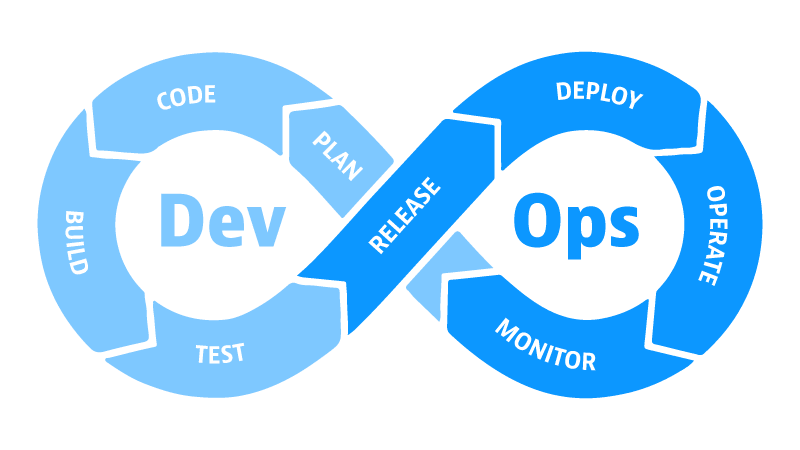
\includegraphics[width=0.7\textwidth]{Images/devops_loop.png}
    \caption{DevOps lifecycle}
    \label{devops_lifecycle}
\end{figure}

In summary, the application of DevOps in this thesis demonstrates how modern software engineering practices can be applied to automate and streamline the testing process, leading to more robust,
efficient and reliable software solutions.

\section{\acrfull{ci}}

\section{Code quality}
\chapter{Creation of Framework}
%Create a flowchart explaining the steps in the framework
%Explain each section in detail
%Explain creation of retrieving the input files using FAST API and OpenShift
%Explain storing of the framework in GitHub
%In this chapter, we will discuss the creation of the framework, steps involved and the implementation of it.

\section{Concept of \acrshort{ci} Framework}
Before, building a framework, it is essential to understand the requirements and objectives of the project. The main objective of this framework is to 
automate the process of running parametric simulations in Optislang, standardize and to verify the output files generated. The framework should be user-friendly,
easy to use, and provide detailed error logs in case of any issues.

After understanding the requirements, the next step is to design the framework. The framework should be designed in such a way that it is scalable,
modular, and easy to maintain. It should also be flexible enough to accommodate future changes and updates. 

This framework is constructed using classes, functions, and libraries such as \verb|Pandas|\footnote{\url{https://pandas.pydata.org}}, \verb|NumPy|\footnote{\url{https://numpy.org}}, 
and other built-in Python modules. Figure \ref{flowchart} provides an overview of the structure and functionality of the framework.
\newpage
%#Creation of flowchart using tikz
\begin{figure}[!ht]
    \centering
      \usetikzlibrary{shapes.geometric, arrows}
      \tikzstyle{box} = [rectangle, rounded corners, minimum width=3cm, minimum height=1.5cm, text centered, text width = 5cm, draw=black, fill=gray!8]
      \tikzstyle{io} = [trapezium, trapezium left angle=70, trapezium right angle=110, minimum width=3cm, minimum height=1cm, text centered, draw=black, fill=blue!30]
      \tikzstyle{image} = [minimum width=3cm, minimum height=1cm, text centered, text width = 2cm]
      \tikzstyle{process} = [rectangle, minimum width=3cm, minimum height=1cm, text centered, draw=black, fill=orange!30]
      \tikzstyle{decision} = [diamond, minimum width=3cm, minimum height=1cm, text centered, draw=black, fill=red!90, text = white]
      \tikzstyle{arrow} = [thick,->,>=stealth]
      \vspace{2cm}
    \begin{tikzpicture}[node distance=2.5cm]
        \node (clone_module) [image] {\centering 
\includegraphics[width=2cm]{Logo/github-mark.pdf}\newline Clone module};
        \node (check_json_files) [decision, below of = clone_module, yshift = -1.5cm] {\textbf{Check JSON Files}};
        \node (yes) [process, right of = check_json_files, xshift = 3cm] {\textbf{Yes}};
        \node (no) [process, left of = check_json_files, xshift = -3cm] {\textbf{No}};
        \node (create_parameters) [box, below of = yes] {\textbf{Create Parameters}};
        \node (get_input_files) [box, below of = create_parameters] {\textbf{Get Input Files}};
        \node (parametric_system) [box, below of = get_input_files] {\textbf{Create and run Parametric System}};
        \node (verify) [box, below of = parametric_system] {\textbf{Verify Output files}};
        \node (error_log) [box, below of = no] {\textbf{Display error : JSON files not found}};

        \draw [arrow] (clone_module) -- (check_json_files);
        \draw [arrow] (check_json_files) -- (yes);
        \draw [arrow] (yes) -- (create_parameters);
        \draw [arrow] (create_parameters) -- (get_input_files);
        \draw [arrow] (get_input_files) -- (parametric_system);
        \draw [arrow] (parametric_system) -- (verify);

        \draw [arrow] (check_json_files) -- (no);
        \draw [arrow] (no) -- (error_log);

    \end{tikzpicture}
    \caption{Flowchart of the framework}
    \label{flowchart}
\end{figure}

Let us understand the working of the framework in detail. The framework is mainly built using Python and uses Optislang's Python API to create and run the 
parametric simulations. The primary requirement for the framework to run is to have the module present. Therefore, the first step is to clone the required module
from the specific repository and branch from GitHub. These serve as the main arguments needed to run the framework. After cloning the module, the framework checks for 
\texttt{module\_config.json} and \texttt{parameters.json} files. These \acrshort{json} files are crucial to be present in the module as they contain the 
information required to run the parametric simulations automatically. The \texttt{module\_config.json} file contains information of 
the module like description of the module, name of the main script containing the algorithm, type of framework, input and output files and their properties.These data are important 
to create, run and verify the parametric system generated. The \texttt{parameters.json} file contains information about the parameters required to be set as input 
in the parametric system.

At this stage, a decision is implemented. If the \acrshort{json} files are present, the framework proceeds to further steps. If the \acrshort{json} files are not found, the framework
comes to a halt and displays an error message being shown to the user. Code snippet \ref{error_message} shows the implementation of the error message. This function is present
inside the class \texttt{ParametricSystem}.
\begin{figure}[!ht]
    \centering
    \renewcommand{\lstlistingname}{Code}
    \lstset{style=pythoncode}
    \begin{lstlisting}[language=python, caption= Function to verify existance of \acrshort{json} files, label={error_message}]
def json_files_log(self):
    try:
        if not self.get_module_config_path().exists():
            raise FileNotFoundError(
                f"{self.get_module_config_path()} does not exist"
            )
    except FileNotFoundError as e:
        print(
            f"{e} \nPlease ensure {self.get_module_config_path()} exists and re-run"
        )
    except Exception as e:
        print(e)
    try:
        if not self.get_parameters_path().exists():
            raise FileNotFoundError(f"{self.get_parameters_path()} does not exist")
    except FileNotFoundError as e:
        print(f"{e} \nPlease ensure {self.get_parameters_path} exists and re-run")
    except Exception as e:
        print(e)
\end{lstlisting}
\end{figure}

If the framework identifies the \acrshort{json} files, it proceeds to the next step of generating the necessary parameters for running the parametric system. 
These parameters are generated in the form of a \texttt{csv} file and a Python file. These files are fed as input to the parametric system. 

The next step is to provide input files which are required by the parametric system in order to execute the simulations. These input files are retrieved from 
a cloud storage using API calls. A more detailed explanation of this process is provided in Section \ref{retrieve_input_files}. 

After the input files are retrieved, the framework proceeds to create the parametric system. This is achieved without the user's intervention, i.e, 
automatically. At this stage, the Python interpreter provided by Optislang is executed as it includes the necessary libraries and functions to create and run 
the parametric system. Another terminal emerges, displaying the progress of the module creation.

Since the whole process in the framework is automated, we need to ensure that the files generated by the parametric system are correct and are produced as 
expected. This is done by the function \texttt{verify\_output\_files} present in the class \texttt{ParametricSystem}. 

A high level overview of the framework is provided in Section \ref{implementation_framework} which provides the functions and classes used in it. 
\section{Directory Structure} \label{directory_structure_section}
The directory structure is depicted in Figure \ref{directory_structure}. The framework consists of the following files and directories:
\begin{itemize}
    \item \textbf{\texttt{moo\_framework\_workflow.yaml}}:\newline
    This file contains the workflow for running the framework automatically. It is written in \acrshort{yaml} and is later used inside GitHub Actions.
    %! Add the reference to the section where the workflow is explained
    \item \textbf{\texttt{src}}:\newline
    This directory contains the source code of the framework. It consists of files which are used to create and run the parametric system in Optislang. It also
    consists of some helper functions which are used to build complex functions and classes for the creation of framework. We will discuss more about these files
    in section %! Add the reference to the section where the files are explained
    .
    \item \textbf{\texttt{tests}}:\newline
    This directory contains test cases for the framework. Section %! Add the reference to the section where the tests are explained
    explains the test cases in detail.
    \item \textbf{\texttt{main.py}}:\newline
    This python file calls the files which are responsible for the framework creation from  \texttt{src} directory . It is the main file for running the framework.
    \item \textbf{\texttt{requirements.txt}}:\newline
    This file contains the list of libraries which helps in running the framework. It is important to install these libraries before running the framework.
\end{itemize}
\newpage
\begin{figure}[!ht]
  \centering
  \newcommand{\githubicon}{
\includegraphics[height=0.4cm]{Logo/github-mark.pdf}}
  \newcommand{\foldericon}{
\includegraphics[height=0.4cm]{Logo/folder_icon.pdf}}
  \newcommand{\pythonicon}{
\includegraphics[height=0.5cm]{Logo/python-logo-only.pdf}}
  \newcommand{\txticon}{
\includegraphics[height=0.5cm]{Logo/txt-svgrepo-com.pdf}}
  \newcommand{\ymlicon}{
\includegraphics[height=0.5cm]{Logo/GitHub Actions.pdf}}

  \begin{forest}
    for tree={
      font=\ttfamily,
      grow'=0,
      child anchor=west,
      parent anchor=south,
      anchor=west,
      calign=first,
      edge path={
        \noexpand\path [draw, \forestoption{edge}]
        (!u.south west) +(7.5pt,0) |- node[fill,inner sep=1.25pt] {} (.child anchor)\forestoption{edge label};
      },
      before typesetting nodes={
        if n=1
          {insert before={[,phantom]}}
          {}
      },
      fit=band,
      before computing xy={l=15pt},
    }
  [MOO Module Framework, label={right:\githubicon}
    [.github, label={right:\foldericon}
      [workflows, label={right:\foldericon}
        [moo\_framework\_workflow.yaml, label={right:\ymlicon}]
      ]
    ]
    [src
      [\_\_init\_\_.py, label={right:\pythonicon}]
      [create\_parametric\_system.py, label={right:\pythonicon}]
      [input\_files.py, label={right:\pythonicon}]
      [parametric\_system.py, label={right:\pythonicon}]
      [run\_parametric\_system.py, label={right:\pythonicon}]
      [utils.py, label={right:\pythonicon}]
    ]
    [tests
      [tests.py, label={right:\pythonicon}]
    ]
    [main.py, label={right:\pythonicon}]
    [requirements.txt, label={right:\txticon}]
  ]
  \end{forest} 
  \caption{Directory structure of the framework}
  \label{directory_structure}
\end{figure}

\section{Testing of \acrshort{ci} Framework}
While building the framework, it is also essential to test the framework to ensure that it is working as expected. One way to do is to include breakpoints, add print 
statements, and debug the code. However, this method is not efficient when the codebase is huge. Therefore, another way is to write unit cases for the framework.

Unit testing is a software testing method that involves testing a small unit of code, typically a function or method. They are crucial part of the development 
process as they help in identifying bugs and errors early in the development cycle. Python has two frameworks for unit testing, \texttt{unittest} and 
\texttt{pytest}. In this thesis,\texttt{unittest} is used for testing since it is part of the Python's standard library. Here, the unit tests can be found 
in the \texttt{tests} directory. The file \texttt{tests.py} contains the test cases for the framework. %Unit tests generally should cover the following aspects:
%# Only mention what test are implemented and why
Boundary tests, negative tests, and unit tests are implemented in the framework. Boundary tests are implemented to check the edge cases of the functions. Here, 
a test function is implemented to verify whether the generated parameters for the system is empty or not. Negative tests are implemented to check if the function 
handles incorrect input properly. To verify the data types generated in the output file, a test case is implemented. This test verifies if the data types in 
the columns of the output file are generated correctly. 
\begin{comment}
\begin{itemize}
  \item \textbf{Unit tests}:\newline
  This is used to test the functionalities of each individual methods and functions.
  \item \textbf{Integration tests}:\newline
  These tests are implemented to verify the interaction of units, modules or components of an application .
  \item \textbf{Boundary tests}:\newline
  This ensures to check the edge cases of the functions. For example, if the provided input is an empty string, the function should return an error message.
  \item \textbf{Negative tests}:\newline
  To check if the function handles incorrect input properly, negative tests are implemented. An example for this would be to handle if the argument is of a 
  different data type than expected. 
\end{itemize}
\end{comment}

Code snippet \ref{unittest} shows an example of a unit test implemented in Python to test the existence of \acrshort{json} files. 
\renewcommand{\lstlistingname}{Code}
\begin{lstlisting}[style=pythoncode, caption={Example of a unit test}, label={unittest}]
class TestParametricSystem(unittest.TestCase):
    def setUp(self) -> None:
        self.parametric_system = ParametricSystem('MOO_M_ARRHENIUS','MOO-1355_py_framework_poc')
        self.cwd = os.getcwd()

    def get_module_name(self):
        for file_name in os.listdir(self.cwd):
            if file_name.startswith('MOO'):
                return Path(self.cwd,file_name)
        return None

    def test_get_module_config_path(self):
        self.assertIsNotNone(self.get_module_name(), 'Module folder not found.')
        expected_path = (Path(self.get_module_name(),'01_Specification', 'module_config.json'))
        actual_path = self.parametric_system.get_module_config_path()
        self.assertEqual(expected_path, actual_path)  
\end{lstlisting}

First, a class \texttt{TestParametricSystem} is created, which inherits from \texttt{unittest.TestCase}. To avoid initialization of the same variables in each
test case, \textbf{\texttt{setUp()}} method is used. Here, an object is created to initialize the arguments for the class \texttt{ParametricSystem}.
The functions in the unit tests needs to start with the prefix \texttt{test}. This convention is used to identify the function which the test cases. For example, 
in Figure \ref{unittest},the function \texttt{test\_get\_module\_config\_path} recognizes that it is a test case whereas the function \texttt{get\_module\_name}
is a helper function and not a test case. In this example, the function \texttt{test\_get\_module\_config\_path} is responsible to check if the path of the folder
containing the \acrshort{json} file is correct or not. To ensure this, \texttt{assertEqual} is used, which checks if the expected path is equal to the 
actual path. If the paths are equal, the test case passes, else it fails. \texttt{unittest} provides several other functions to test the code. 

\section{Execution of \acrshort{ci} Framework}
To execute the framework, the user needs to run the file \texttt{main.py}. This script calls the functions
from the class \texttt{ParametricSystem} and runs the module.


An instance of the class \texttt{ParametricSystem} 
is created with the arguments \texttt{module\_name} and \texttt{module\_branch\_name}. Then, the check for the \texttt{\acrshort{json}} files is done. 
The verifying of the files is done outside the function \texttt{run\_module()} as we do need to verify the existence of the files before running the module.
Once the existence of the files are verified, the module is being run and after the successful execution in Optislang, it displays the status of the output
files. 

This framework also contains some external libraries which are required for the functioning of the framework. Therefore, \texttt{requirements.txt} file contains the list of libraries
required to install before running the framework in the virtual machine. Execution of the framework is provided in detail with an example in Chapter \ref{results}.

\section{Tools used in the \acrshort{ci} Framework} \label{retrieve_input_files}
Input files which are required by the module can be mocked using the data in \texttt{module\_config.json}. But, in some modules, the input files required are very complex. For example, the module, \texttt{ROM SOLVER}, needs input files in the form of 
matrices, containing 250,000 lines of data. Mocking these huge files is time consuming, inefficient and not a way to standardize the framework. Therefore,
the idea was to save these files in a cloud storage and retrieve them later when required. This improves the efficiency of the framework and also helps in
standardizing it. 

To store the input files, OpenShift is used. OpenShift\cite{openshift} is a Kubernetes platform which helps in deploying, scaling and managing containerized applications. 
OpenShift is used in this thesis as it is easy to build, deploy and maintain in the cloud. The application in OpenShift needs to be containerized and deployed. 

Docker\cite{docker} is a platform for developing, shipping and running applications effectively. It is a containerization platform which packages the application and all 
its dependencies together in the form of containers. Docker is preferred for development and deployment as it is lightweight, portable and scalable. This can 
run anywhere, regardless of the operating system. 
\begin{figure}[!ht]
  \centering
  \tikzstyle{image} = [minimum width=3cm, minimum height=1cm, text centered, text width = 2cm]
  \tikzstyle{arrow} = [thick,->,>=stealth]
  \begin{tikzpicture}[node distance=6cm]
    \node (Dockerfile) [image] {\centering 
\includegraphics[width=2cm]{Images/docker.pdf}\newline Dockerfile};
    \node (Dockerimage) [image, right of = Dockerfile] {\centering 
\includegraphics[width=2cm]{Images/docker_image.pdf} \newline Docker Image};
    \node (Dockercontainer) [image, right of = Dockerimage] {\centering 
\includegraphics[width=2cm]{Images/container.pdf} \newline Docker Container};

    \draw [arrow] (Dockerfile) -- node[anchor=south] {Build} (Dockerimage);
    \draw [arrow] (Dockerimage) -- node[anchor=south] {Run} (Dockercontainer);
  \end{tikzpicture}
  \caption{Creation and deployment of Docker image}
  \label{docker_image_creation}
\end{figure}

To build an image in Docker, a Dockerfile is required. The Dockerfile contains the instructions to build the Docker image. Figure \ref{docker_image_creation} 
shows the creation of a container. This container contains input files required for modules to run the parametric system in Optislang. 

But, the input files are not directly accessible from the container. To transfer the files, a communication medium is required. This is achieved by using 
\acrshort{api} calls. \acrshort{api} is a collection of protocols and tools which allows different software applications to communicate with each other.
Figure \ref{api_working} shows the working of an \acrshort{api}. 
\newpage
\begin{figure}[!ht]
  \centering
  \tikzstyle{image} = [minimum width=3cm, minimum height=1cm, text centered, text width = 2cm]
  \tikzstyle{arrow} = [thick,->,>=stealth]
  \begin{tikzpicture}[node distance=7cm]
    \node (client) [image] {\centering 
\includegraphics[width=2.5cm]{Images/computer-coding.pdf} \newline Client};
    \node (api)  [image, right of = client] {\centering 
\includegraphics[width=2.5cm]{Images/api.pdf} \newline API};
    \node (server) [image, right of = api] {\centering 
\includegraphics[width=2.5cm]{Images/database.pdf} \newline Server};

    \path (client.east) -- (client.north east) coordinate[pos=0.2] (client1);
    \path (api.west) -- (api.north west) coordinate[pos=0.2] (api1);
    \draw[latex-] (client1) -- (api1) node[midway, above] {Response};

    \path (api.east) -- (api.north east) coordinate[pos=0.2] (api2);
    \path (server.west) -- (server.north west) coordinate[pos=0.2] (server1);
    \draw[latex-] (api2) -- (server1);

    % Response Arrow coordinates (Server -> API -> Client) on the bottom
    \path (server.west) -- (server.south west) coordinate[pos=0.1] (server2);
    \path (api.east) -- (api.south east) coordinate[pos=0.1] (api3);
    \draw[latex-] (server2) -- (api3);

    \path (api.west) -- (api.south west) coordinate[pos=0.1] (api4);
    \path (client.east) -- (client.south east) coordinate[pos=0.1] (client2);
    \draw[latex-] (api4) -- (client2) node[midway, below] {Request};
  \end{tikzpicture}
  \caption{Working of an \acrshort{api}}
  \label{api_working}
\end{figure}

An \acrshort{api} takes the request from the client, processes it and sends the response to the server. The server processes the request and sends the required 
information back to the client. This thesis leverages the use of \acrshort{api} to request for input files from the cloud storage. To build the \acrshort{api},
Fast\acrshort{api} is used. Fast\acrshort{api}\cite{fastapi} is a modern, fast (high-performance), web framework for building \acrshort{api} with Python. Fast\acrshort{api} 
is preferred as it is easy to use, fast to develop, high performance and easy to deploy. To secure the \acrshort{api} calls and to access the input files, a basic \acrshort{http}  
authentication is implemented in this thesis. Figure \ref{directory_structure_input_files} shows the file structure of the input files storage.
\newpage
\begin{figure}[!ht]
  \centering
  \newcommand{\githubicon}{
\includegraphics[height=0.4cm]{Logo/github-mark.pdf}}
  \newcommand{\foldericon}{
\includegraphics[height=0.4cm]{Logo/folder_icon.pdf}}
  \newcommand{\pythonicon}{
\includegraphics[height=0.5cm]{Logo/python-logo-only.pdf}}
  \newcommand{\txticon}{
\includegraphics[height=0.5cm]{Logo/txt-svgrepo-com.pdf}}
  \newcommand{\dockericon}{
\includegraphics[height=0.5cm]{Images/docker.pdf}}
  \newcommand{\envicon}{
\includegraphics[height=0.5cm]{Logo/settings-svgrepo-com.pdf}}

  \begin{forest}
    for tree={
      font=\ttfamily,
      grow'=0,
      child anchor=west,
      parent anchor=south,
      anchor=west,
      calign=first,
      edge path={
        \noexpand\path [draw, \forestoption{edge}]
        (!u.south west) +(7.5pt,0) |- node[fill,inner sep=1.25pt] {} (.child anchor)\forestoption{edge label};
      },
      before typesetting nodes={
        if n=1
          {insert before={[,phantom]}}
          {}
      },
      fit=band,
      before computing xy={l=15pt},
    }
  [Input Files Storage, label={right:\foldericon}
    [src, label={right:\foldericon}
      [routers, label={right:\foldericon}
        [\_\_init\_\_.py, label={right:\pythonicon}]
        [files.py, label={right:\pythonicon}]
      ]
      [file.py, label={right:\pythonicon}]
      [security.py, label={right:\pythonicon}]
    ]
    [static-files
      [arrhenius, label={right:\foldericon}]
      [coffin\_manson, label={right:\foldericon}]
      [pv\_calculator, label={right:\foldericon}]
      [rainflow\_counting, label={right:\foldericon}]
      [rom\_solver, label={right:\foldericon}]
      [rom\_solver\_prepro, label={right:\foldericon}]
    ]
    [main.py, label={right:\pythonicon}]
    [requirements.txt, label={right:\txticon}]
    [Dockerfile, label={right:\dockericon}]
    [.env, label={right:\envicon}]
  ]
  \end{forest} 
  \caption{Directory structure of the input files storage}
  \label{directory_structure_input_files}
\end{figure}

\texttt{src} contains the scripts needed to establish a connection with Fast\acrshort{api}. Fast\acrshort{api} contains two \texttt{GET} endpoints which helps in the retrieval of
input files. Endpoint \texttt{getInputFiles} returns a dictionary containing the key-value pair of module name and the corresponding location of the input 
files. The directory \texttt{static-files} contains the input files which is used to retrieve the input files. The endpoint \texttt{download} takes the location 
of a file as an argument and returns the file to the user.

To access the input files in a cloud storage, we build a docker image consisting of the Fast\acrshort{api} implementation and the input files. Code snippet 
\ref{dockerfile} shows the creation of an image using Dockerfile. 
\renewcommand{\lstlistingname}{Code}
\begin{lstlisting}[language=Dockerfile ,caption={Implementation of Dockerfile}, label={dockerfile}]
FROM python:3.10
WORKDIR /code

COPY ./requirements.txt /code/
COPY ./static-files/ /code/static-files/

RUN ["python", "-m", "pip", "install", "-r", "requirements.txt"]

EXPOSE 7000

RUN mkdir -p ./temp && \
    chgrp -R 0 ./temp && \
    chmod -R g=u ./temp

COPY main.py /code/
COPY ./src/ /code/src/
COPY .env /code/.env
ENTRYPOINT ["python", "-m", "uvicorn", "main:app", "--host", "0.0.0.0", "--port", "7000"]
\end{lstlisting}

The Dockerfile contains the instructions to build the Docker image. Here, the Dockerfile copies the folder containing the input files and Fast\acrshort{api}.
It installs the required libraries using the \texttt{requirements.txt} file. Later, it exposes the port 7000 and runs the Fast\acrshort{api} using the
uvicorn server in OpenShift. This is later used during the first step of executing the parametric system.

The \texttt{.env} file contains the environment variables consisting of authentication details to access the \acrshort{api}. 
\begin{comment}

\subsection{Docker}
Docker is platform used for developing, shipping and running applications effectively. It is a containerization platform which packages the application and 
all its dependencies together in the form of containers. To run Docker in a local machine or in a cloud, we need to install it. Docker is preferred during
development and deployment as it is lightweight, portable and scalable. This can run anywhere, regardless of the operating system.
\begin{figure}[!ht]
  \centering
  \tikzstyle{image} = [minimum width=3cm, minimum height=1cm, text centered, text width = 2cm]
  \tikzstyle{arrow} = [thick,->,>=stealth]
  \begin{tikzpicture}[node distance=6cm]
    \node (Dockerfile) [image] {\centering 
\includegraphics[width=2cm]{Images/docker.pdf}\newline Dockerfile};
    \node (Dockerimage) [image, right of = Dockerfile] {\centering 
\includegraphics[width=2cm]{Images/docker_image.pdf} \newline Docker Image};
    \node (Dockercontainer) [image, right of = Dockerimage] {\centering 
\includegraphics[width=2cm]{Images/container.pdf} \newline Docker Container};

    \draw [arrow] (Dockerfile) -- node[anchor=south] {Build} (Dockerimage);
    \draw [arrow] (Dockerimage) -- node[anchor=south] {Run} (Dockercontainer);
  \end{tikzpicture}
  \caption{Creation and deployment of Docker image}
  \label{docker_image_creation}
\end{figure}
A Dockerfile contains instructions to build a Docker image. It is basically a blueprint to built the Docker image. A Docker image is a lightweight, standalone, 
executable package that includes everything needed to run the application. WHen the image is run, it becomes a container. Figure \ref{docker_image_creation}
shows the creation and deployment of a Docker image. 

The main difference between a docker container and a virtual machine is that a container shares the host's kernel which makes it more lightweight and faster.
Whereas, a virtual machine reserves some place in the host's memory for the guest operating system, libraries and applications which makes it slower and heavier.

\subsection{OpenShift}
%# Intro to OpenShift


\begin{figure}[!ht]
  \centering
  \tikzstyle{image} = [minimum width=3cm, minimum height=1cm, text centered, text width = 2cm]
  \tikzstyle{arrow} = [thick,->,>=stealth]
  \begin{tikzpicture}[node distance=7cm]
    \node (client) [image] {\centering 
\includegraphics[width=2.5cm]{Images/computer-coding.pdf} \newline Client};
    \node (api)  [image, right of = client] {\centering 
\includegraphics[width=2.5cm]{Images/api.pdf} \newline API};
    \node (server) [image, right of = api] {\centering 
\includegraphics[width=2.5cm]{Images/database.pdf} \newline Server};

    \path (client.east) -- (client.north east) coordinate[pos=0.2] (client1);
    \path (api.west) -- (api.north west) coordinate[pos=0.2] (api1);
    \draw[latex-] (client1) -- (api1) node[midway, above] {Response};

    \path (api.east) -- (api.north east) coordinate[pos=0.2] (api2);
    \path (server.west) -- (server.north west) coordinate[pos=0.2] (server1);
    \draw[latex-] (api2) -- (server1);

    % Response Arrow coordinates (Server -> API -> Client) on the bottom
    \path (server.west) -- (server.south west) coordinate[pos=0.1] (server2);
    \path (api.east) -- (api.south east) coordinate[pos=0.1] (api3);
    \draw[latex-] (server2) -- (api3);

    \path (api.west) -- (api.south west) coordinate[pos=0.1] (api4);
    \path (client.east) -- (client.south east) coordinate[pos=0.1] (client2);
    \draw[latex-] (api4) -- (client2) node[midway, below] {Request};
  \end{tikzpicture}
  \caption{Working of an \acrshort{api}}
  \label{api_working}
\end{figure}


\subsection{Implementation}
%# Explain the implementation of retrieving input files using Fast API and OpenShift
After understanding the practices and tools, we will discuss the implementation of retrieving the input files from OpenShift using Fast\acrshort{api}.
To access the input files remotely, we need to upload a docker image to OpenShift. The docker image contains the implementation of Fast\acrshort{api} and 
the input files required for the parametric system. To access the input files, we need to create endpoints in Fast\acrshort{api}. Figure \ref{directory_structure_input_files}
shows the directory structure of the input files storage.
\newpage
\begin{figure}[!ht]
  \centering
  \newcommand{\githubicon}{
\includegraphics[height=0.4cm]{Logo/github-mark.pdf}}
  \newcommand{\foldericon}{
\includegraphics[height=0.4cm]{Logo/folder_icon.pdf}}
  \newcommand{\pythonicon}{
\includegraphics[height=0.5cm]{Logo/python-logo-only.pdf}}
  \newcommand{\txticon}{
\includegraphics[height=0.5cm]{Logo/txt-svgrepo-com.pdf}}
  \newcommand{\dockericon}{
\includegraphics[height=0.5cm]{Images/docker.pdf}}
  \newcommand{\envicon}{
\includegraphics[height=0.5cm]{Logo/settings-svgrepo-com.pdf}}

  \begin{forest}
    for tree={
      font=\ttfamily,
      grow'=0,
      child anchor=west,
      parent anchor=south,
      anchor=west,
      calign=first,
      edge path={
        \noexpand\path [draw, \forestoption{edge}]
        (!u.south west) +(7.5pt,0) |- node[fill,inner sep=1.25pt] {} (.child anchor)\forestoption{edge label};
      },
      before typesetting nodes={
        if n=1
          {insert before={[,phantom]}}
          {}
      },
      fit=band,
      before computing xy={l=15pt},
    }
  [Input Files Storage, label={right:\foldericon}
    [src, label={right:\foldericon}
      [routers, label={right:\foldericon}
        [\_\_init\_\_.py, label={right:\pythonicon}]
        [files.py, label={right:\pythonicon}]
      ]
      [file.py, label={right:\pythonicon}]
      [security.py, label={right:\pythonicon}]
    ]
    [static-files
      [arrhenius, label={right:\foldericon}]
      [coffin\_manson, label={right:\foldericon}]
      [pv\_calculator, label={right:\foldericon}]
      [rainflow\_counting, label={right:\foldericon}]
      [rom\_solver, label={right:\foldericon}]
      [rom\_solver\_prepro, label={right:\foldericon}]
    ]
    [main.py, label={right:\pythonicon}]
    [requirements.txt, label={right:\txticon}]
    [Dockerfile, label={right:\dockericon}]
    [.env, label={right:\envicon}]
  ]
  \end{forest} 
  \caption{Overview of implementation of retrieving input files}
  \label{directory_structure_input_files}
\end{figure}

\texttt{src} contains the scripts needed to establish a connection with Fast\acrshort{api}. Fast\acrshort{api} contains two \texttt{GET} endpoints which helps in the retrieval of
input files. Endpoint \texttt{getInputFiles} returns a dictionary containing the key-pair value of module name and the corresponding location of the input 
files. The directory \texttt{static-files} contains the input files which is used to retrieve the input files. The endpoint \texttt{download} takes the location 
of a file as an argument and returns the file to the user.

To access the input files in a cloud storage, we build a docker image consisting of the Fast\acrshort{api} implementation and the input files. Figure
\ref{dockerfile} shows the implementation of the Dockerfile. 
\renewcommand{\lstlistingname}{Code}
\begin{lstlisting}[language=Dockerfile ,caption={Implementation of Dockerfile}, label={dockerfile}]
FROM python:3.10
WORKDIR /code

COPY ./requirements.txt /code/
COPY ./static-files/ /code/static-files/

RUN ["python", "-m", "pip", "install", "-r", "requirements.txt"]

EXPOSE 7000

RUN mkdir -p ./temp && \
    chgrp -R 0 ./temp && \
    chmod -R g=u ./temp

COPY main.py /code/
COPY ./src/ /code/src/
COPY .env /code/.env
ENTRYPOINT ["python", "-m", "uvicorn", "main:app", "--host", "0.0.0.0", "--port", "7000"]
\end{lstlisting}

The Dockerfile contains the instructions to build the Docker image. Here, the Dockerfile copies the folder containing the input files and Fast\acrshort{api}.
It installs the required libraries using the \texttt{requirements.txt} file. Later, it exposes the port 7000 and runs the Fast\acrshort{api} using the
uvicorn server. The \texttt{.env} file contains the environment variables consisting of username and password to access the \acrshort{api}. 

After building the Docker image, it is deployed in a pod in OpenShift. Using OpenShift, we can access the input files remotely via \acrshort{api} calls. This 
is later called during the first step of creating the parametric system.
\end{comment}

%!\section{Summary}
%# Create a flowchart explaining the final working of the framework using all the tools and practices
\chapter{Implementation of CI Pipeline} \label{ci_pipeline}
\section{Introduction}
%# What is it?
%# Uses
%# Where is it used in my thesis?
\section{GitHub Actions}
%# What is it?
%# Uses and advantages
\section{Running the pipeline}
%# Using it in the framework
\chapter{Results} \label{results}

This chapter presents the results of the experiments conducted in the previous chapters. The results are present with an example of execution of a standalone 
module in Optislang.  

\texttt{ARRHENIUS} module is responsible for calculating the field load equivalent hours according to Arrhenius lifetime model for each relevant monitor point
in the design. To run this module, the developer needs to execute \texttt{main.py}, providing the module name and name of the branch where the module is present.
Code snippet \ref{main_script} provides the code for executing the framework using \texttt{main.py}.

\renewcommand{\lstlistingname}{Code}
\begin{lstlisting}[style=pythoncode, caption={Execution of framework using \texttt{main.py}}, label={main_script}]
from src import ParametricSystem

module_name = "MOO_M_ARRHENIUS"
module_branch_name = 'MOO-1355_py_framework_poc'

def main():
    system = ParametricSystem(module_name, module_branch_name)
    system.clone_module()
    if (
        system.get_module_config_path().exists() & system.get_parameters_path().exists()
    ) == True:
        system.run_module()
        system.verify_output_file()

    else:
        system.json_files_log()

if __name__ == "__main__":
    main()
\end{lstlisting}

\texttt{main.py} calls the \texttt{ParametricSystem} class containing the framework. After cloning the module, the framework verifies the existence of the 
\texttt{\acrshort{json}} files. If the files are not present, the framework provides a log message to the user.

\renewcommand{\lstlistingname}{Code}
\begin{lstlisting}[style=terminal, caption=Error message when \acrshort{json} files are not present, label={json_files_log}]
c:\Users\BIS4SI\Desktop\MOO_Module_Framework\MOO_M_ARRHENIUS\01_Specification\module_config.json does not 
exist 
Please ensure c:\Users\BIS4SI\Desktop\MOO_Module_Framework\MOO_M_ARRHENIUS\01_Specification\module_config.
json exists and re-run
\end{lstlisting}

In code snippet \ref{json_files_log}, the framework provides an error message when the \acrshort{json} file, \texttt{module\_config.json}, is not present.

After verifying the existence of the \acrshort{json} files, the framework continues further to create the required parameters and runs the parametric system.
\begin{figure}[!ht]
    \centering
    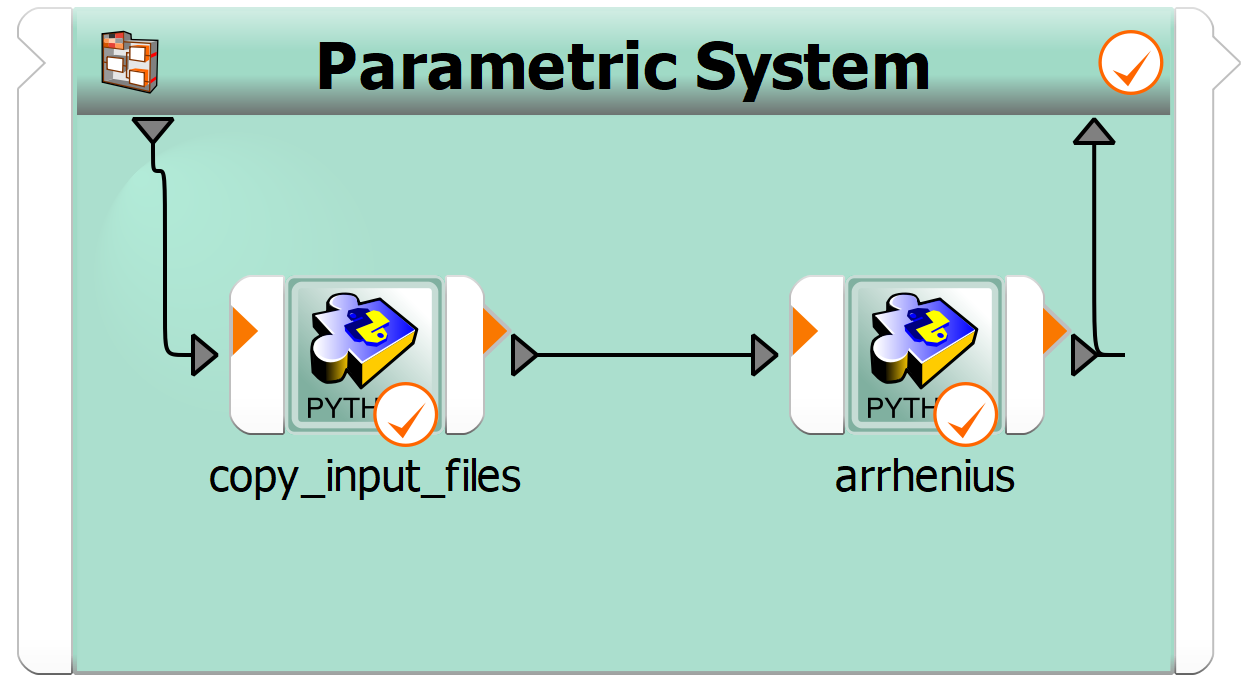
\includegraphics[width=0.5\textwidth]{Images/parametric_system_with_copy_actor.png}
    \caption{Execution of ARRHENIUS module in Optislang}
    \label{parametric_system_with_copy_actor}
  \end{figure}

Figure \ref{parametric_system_with_copy_actor} shows the parametric system created by the framework. The system consists of a python actor, \textbf{copy\_input\_files},
which contains the algorithm to retrieve the input files from OpenShift via \acrshort{api} calls. These input files are stored in the working directory of the 
parametric system. Later, the system continues to run the actor, \texttt{arrhenius}, containing the module. The tick mark on the actors indicate the successful 
execution in Optislang. Successful execution of the parametric system is also displayed in the console as shown in Code snippet \ref{parametric_system_execution}.
\renewcommand{\lstlistingname}{Code}
\begin{lstlisting}[style=terminal, caption=Message providing status of parametric system execution, label={parametric_system_execution}]
Attribute Qt::AA_UseSoftwareOpenGL must be set before QCoreApplication is created.
INFO : Saving project "parametric_system"
INFO : New project "parametric_system". Working dir : "c:\Users\BIS4SI\Desktop\MOO_Module_Framework\MOO_M_
ARRHENIUS\Module\02_Model\parametric_system.opd".
INFO : working directory of "parametric_system" set to "c:\Users\BIS4SI\Desktop\MOO_Module_Framework\MOO_M
_ARRHENIUS\Module\02_Model\parametric_system.opd"
INFO_DETAIL : License feature checkout requested (first of): optislang_level2 [in 281 milliseconds]
INFO_DETAIL : 2024-Sep-30 09:14:07.340325 : License feature checkout requested (first of): optislang_level
2 [in 1 millisecond]
INFO : 2024-Sep-30 09:14:07.340325 : Auto-saving project "parametric_system"
INFO : 2024-Sep-30 09:14:07.409259 : parametric_system : Current iteration successfully prepared
INFO : 2024-Sep-30 09:14:07.409259 : Parametric System : Sent Design 1
INFO : 2024-Sep-30 09:14:07.432607 : Parametric System : Current iteration successfully prepared
INFO : 2024-Sep-30 09:14:11.214374 : copy_input_files : copy_input_files processed successfully [Design 1]
INFO : 2024-Sep-30 09:14:12.848899 : arrhenius : arrhenius processed successfully [Design 1]
INFO : 2024-Sep-30 09:14:12.859403 : Parametric System : Collected Design 1
INFO : 2024-Sep-30 09:14:12.863430 : Parametric System :  Parametric System processed successfully
INFO : 2024-Sep-30 09:14:12.863430 : Auto-saving project "parametric_system"
INFO : 2024-Sep-30 09:14:12.024235 : Auto-saving project "parametric_system"
INFO : 2024-Sep-30 09:14:12.976036 : Auto-saving project "parametric_system"
INFO : 2024-Sep-30 09:14:13.042652 : Total execution time : 6 seconds
INFO : 2024-Sep-30 09:14:13.059409 : Saving project "parametric_system"
\end{lstlisting}

This whole framework is implemented in the \acrshort{ci} pipeline using GitHub Actions. The pipeline is triggered when a developer pushes the code to the 
repository. If all of the steps in the pipeline are successful, new commits are pushed to the branch. If the pipeline fails, the developer is notified via email 
about the failure. This is shown in Figure \ref{github_actions_notification}.
\begin{figure}[!ht]
    \centering
    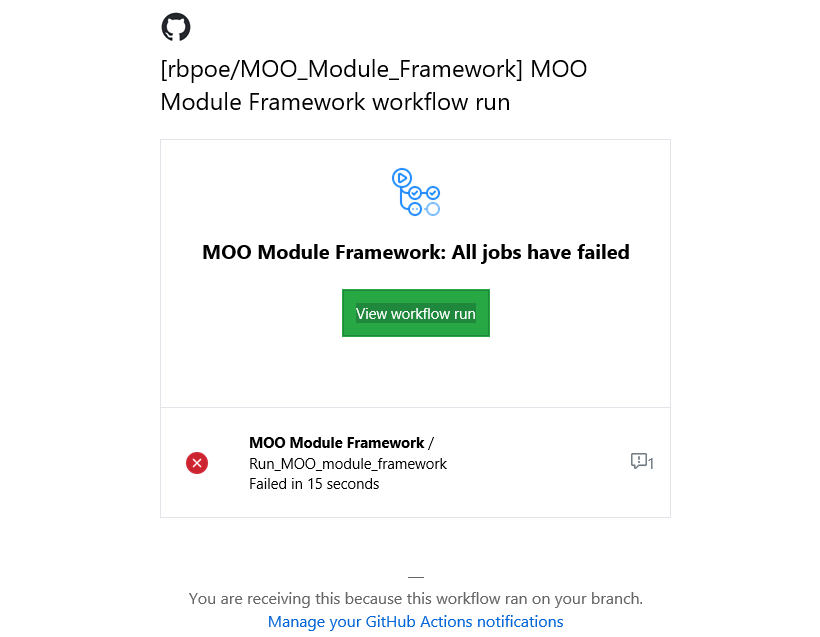
\includegraphics[width=0.8\textwidth]{Images/github_actions_notification.png}
    \caption{Notification of pipeline failure in GitHub Actions}
    \label{github_actions_notification}
\end{figure}

After the successful execution of the system in the pipeline, the framework checks the output file generated by the module. Here, the algorithm checks if the
output file generated is as expected, which is provided in \texttt{module\_config.json}. A detailed explanation verification of output files is provided in 
Section \ref{parametric_system_code}. A detailed log message is provided to the user regarding the output file. Code snippet \ref{output_file_verification} shows the log message provided 
to the user. 
\renewcommand{\lstlistingname}{Code}
\begin{lstlisting}[style=terminal, caption={Log message for output file verification}, label={output_file_verification}]
arrhenius_results.csv present
{'monitoring_point': 'str', 'time': 'float'}
Column 'monitoring_point' not found in arrhenius_results.csv
Column 'time' not found in arrhenius_results.csv
\end{lstlisting}
In Code snippet \ref{output_file_verification}, the algorithm confirms the presence of the output file, \texttt{arrhenius\_results.csv}. But, the column names
\texttt{montoring\_point} and \texttt{time} are not present. If the column names are present, it verifies if the data types of the columns are as expected.

The framework is also responsible for creating and excuting MATLAB modules in Optislang. The developer needs to provide the module name and the branch 
name where the module is present. The framework takes care of the rest of the process. Figure \ref{parametric_system_coffin_manson} shows the successful execution of the MATLAB module, 
\texttt{COFFIN MANSON}, in Optislang. 
\newpage
\begin{figure}[!ht]
    \centering
    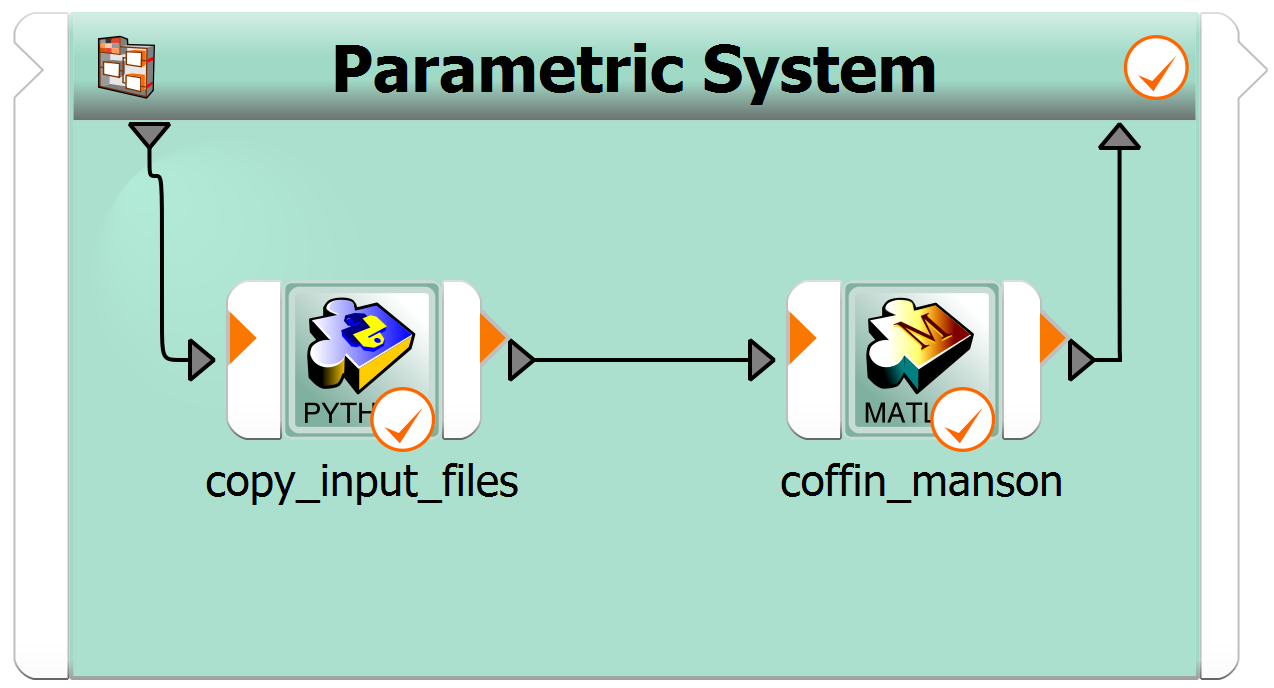
\includegraphics[width=0.5\textwidth]{Images/parametric_system_coffin_manson.png}
    \caption{Execution of MATLAB module in Optislang}
    \label{parametric_system_coffin_manson}
\end{figure}

The execution of the MATLAB modules takes a bit longer compared to the Python module. This is due to execution of MATLAB in the background. 
Currently, the framework is capable of running Python and MATLAB modules. The framework is built in such a way that it can be extended to run other 
modules as well. To run other modules in the framework, the developer only needs to provide the module name and branch of the module. The framework and the 
\acrshort{ci} pipeline take care of the rest of the process.

Earlier, the developer had to manually test their new commits to the module by running the module in Optislang. This process was taking around 30 minutes to 
complete. With the help of the framework, the developer can now run the module in Optislang in seconds. In Code snippet \ref{parametric_system_execution}, the 
framework took around 6 seconds to run the module in Optislang. This is a significant improvement in the time taken to run the module in Optislang compared to the 
manual process. 
\chapter{Summary}
\section{Conclusion}
The goal of this thesis was to develop a \acrlong{ci} framework for Optislang workflows that tests the modules and provides immediate feedback to the developer
without the user intervention. 
By implementing this framework, modules can be tested faster and reduce errors during the development process. Through the implementation of a Python-based framework, 
integrated with GitHub Actions, the workflow has been successfully automated, simplifying the development process for system developers at Bosch

Throughout the project, key efforts were directed toward automating the execution and testing of these modules, which were previously handled manually. 
By incorporating DevOps best practices into the framework, the process has become much more efficient, offering immediate feedback whenever changes are 
pushed to the repository. This not only saves time but also helps minimize human error during development.

The work presented here is particularly relevant as industries increasingly depend on automation to stay competitive. With the growing complexity of modern 
software and optimization tools like OptiSlang, automating repetitive tasks like testing ensures that companies can move faster and deliver more reliable 
products, which is crucial for companies like Bosch.

Ultimately, the takeaway from this thesis is clear: integrating CI practices into simulation-based environments can greatly enhance productivity, reliability, 
and scalability. This work demonstrates how automation can play a vital role in ensuring the success of complex workflows, enabling developers to focus more 
on innovation and less on routine tasks.

\section{Future Work}
The framework developed in this thesis is a starting point for automating Optislang workflows. Future work could focus on expanding the framework to support 
more modules and tools. For example, the framework could be extended to support for workflows that involve multiple modules, or to integrate with other 
optimization tools. Additionally, the framework could be enhanced to support more advanced testing. This changes can be implemented easily by extending the 
functionality of the framework. 

Some of the older modules in the framework do not consist the data for verifying output files. This is a crucial step in the framework to verify the output 
files generated by the module. By standardizing the files in every module, the framework can be used for all the modules in the repository.

Storage of input files in this thesis is done through OpenShift and Fast\acrshort{api} for a proof of concept. This can be improved by using a more secure and 
scalable solution. One possible solution is to store the files in a Blob storage in Azure\footnote{\url{https://azure.microsoft.com/en-us/products/storage/blobs/}}, 
securing the files and making it easier to access the files.
\appendix
\chapter{Appendix}
\section{Implementation of the Framework}
%!+++++++++++++++++++++++++++++++++++++++++++++++++++++++++++++++++++++++++++++++++++++++++++++++++++++++++++++++++++++++
In this section, we will briefly discuss the working and functioning of each of the files present in the framework. Each of the files are crucial and responsible
for the proper functioning and execution of the framework. 

\subsection{Utility files}
During creation of a framework, it is common to repeat functionalities in different parts of the codebase. But, it is frowned upon in software development as 
it leads to code redundancy and makes the codebase difficult to maintain. Therefore, it is ideal to store the repeated functionalities in a separate file and
import them when required. A utility file refers to a Python source file  which contains utility functions or helper functions. These functions are built in a 
way that they can provide common functionalities or operate specific tasks which can be reused in different parts of the codebase. 
\begin{figure}[!ht] %! Image is not being displayed as expected. FIX IT!!!
  \centering
  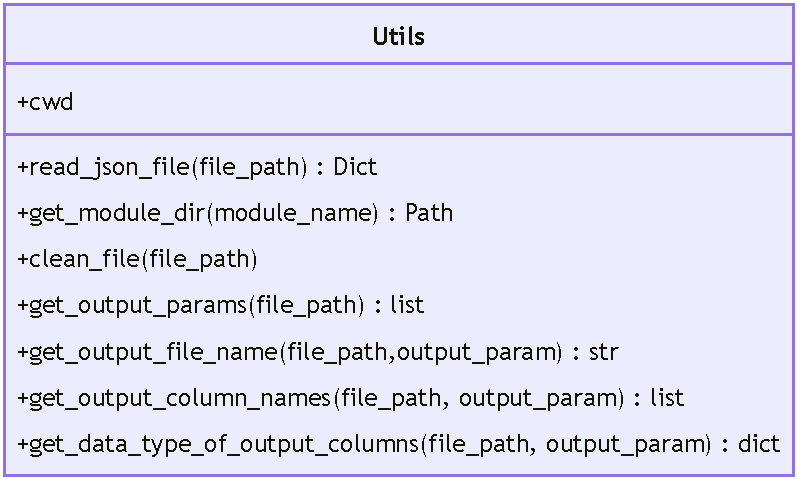
\includegraphics[width=0.6\textwidth]{Images/utils.pdf}
  \caption{Overview of functions in \texttt{utils.py}}

  \label{utils_overview}
\end{figure}

\textbf{\texttt{utils.py}} is a helper file which mainly consists of functions which are later used to build complex functions for the creation of the framework.
It consists of functions like \texttt{read\_json\_file} which reads a \acrshort{json} file and returns the data in the form of dictionary, get the path of a module,
get column names of a \texttt{csv} file, get data type of a column in a \texttt{csv} file and many more. Figure \ref{utils_overview} shows the functions present 
in the \texttt{utils.py} file.

\subsection{Creation and Execution of Parametric System}
Since the main objective of the framework is to automate the process of running parametric simulations in Optislang, it is essential to create the parametric 
system automatically. The script \texttt{create\_parametric\_system.py} assists in creating the parametric system without the help of Optislang's GUI. The 
parametric system is created based on the information present in \texttt{module\_config.json}. The \acrshort{json} file consists of key-value pairs containing 
crucial information for creating the system, like name of the main script containing the algorithm, type of module to build, i.e, Python or MATLAB. 
\begin{figure}[!ht]
  \centering
  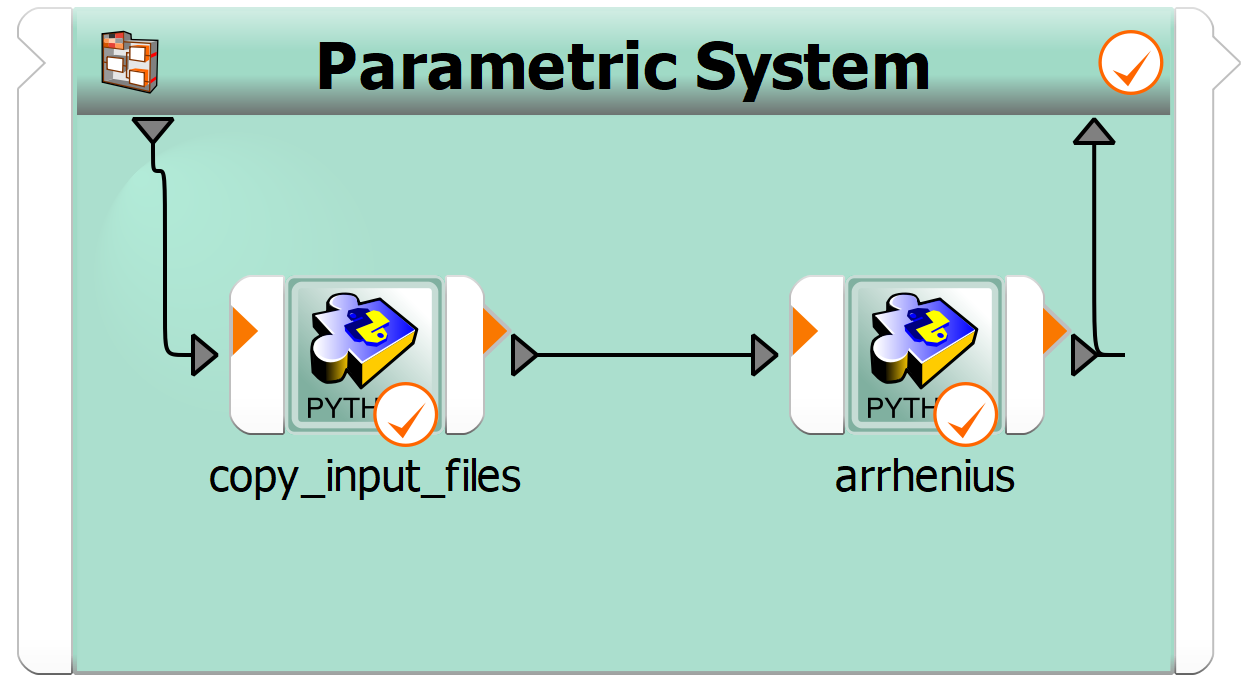
\includegraphics[width=0.5\textwidth]{Images/parametric_system_with_copy_actor.png}
  \caption{Example of a parametric system with copy actor}
  \label{parametric_system_with_copy_actor}
\end{figure}

Optislang takes in different functions to create a system depending on the type of actor. Therefore, type of module is required. Since the framework is automated,
the process of inputting the requried files also needs to be automated. The script \texttt{input\_files.py} is responsible for retrieving the input files from 
OpenShift. A detailed explanation of retrieving input files from OpenShift is provided in Section %! Add the reference to the section where the explanation is provided
After providing the input files, the parametric system is created and is shown in Figure \ref{parametric_system_with_copy_actor}. 

The next step is to run the created parametric system. \texttt{run\_parametric\_system.py} runs the newly created parametric system. This system is being run 
inside the Python interpreter provided by Optislang. These scripts are being called and ran in an orchestrated manner inside the class \texttt{ParametricSystem}.


\subsection{Framework Orchestration}
For better code organization, reusability and encapsulation, the framework is built using classes. Classes are the pillar of object-oriented programming.
There are many advantages of using classes.
\begin{itemize}
  \item Code is maintained and organized in a better way.
  \item Data can be encapsulated and hidden from the user.
  \item Code can be reused and extended easily.
\end{itemize}
Creation of framework is possible by using the class \texttt{ParametricSystem}. Since the creation of framework is tedious and complex, we make use of 
\texttt{utils.py} which assists in building the class. Figure \ref{parametric_system_class} shows the functions present in the class \texttt{ParametricSystem}.
\begin{figure}[!ht]
  \centering
  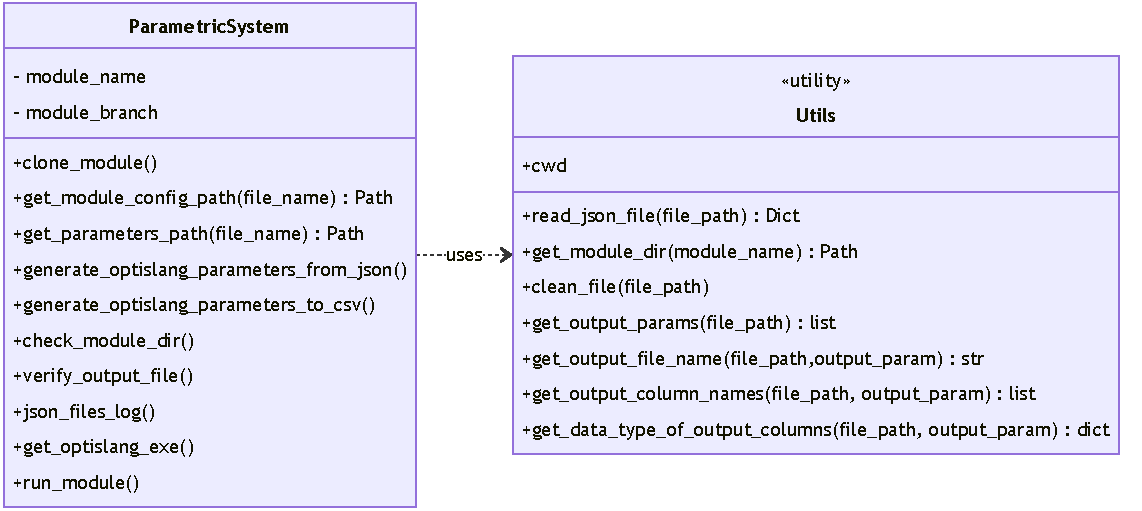
\includegraphics[width=0.9\textwidth]{Images/parametric_system_class.pdf}
  \caption{Overview of the class \texttt{ParametricSystem}}
  \label{parametric_system_class}
\end{figure}

The class takes in the arguments \texttt{module\_name} and \texttt{module\_branch} which are required to clone the module from GitHub. 
The following provides a high-level overview of the key functions used in the framework. These functions are essential for automating the process of testing 
standalone modules in Optislang.

\begin{itemize}
  \item \textbf{\texttt{clone\_module()}}:
  This function is responsible for cloning a module from a GitHub repository. It ensures that any existing module is deleted before cloning the new one, 
  thereby maintaining a clean working environment.

  \item \textbf{\texttt{get\_module\_config\_path()}}:
  This function retrieves the absolute path of the \texttt{module\_config.json} file. It takes the file name as an argument and returns its absolute path, 
  facilitating easy access to the configuration file.

  \item \textbf{\texttt{get\_parameters\_path()}}:
  Similar to \texttt{get\_module\_config\_path()}, this function returns the absolute path of the \texttt{parameters.json} file. It ensures that the framework 
  can locate and use the parameters file efficiently.

  \item \textbf{\texttt{generate\_optislang\_parameters\_to\_csv()}}:
  This function converts the parameters from the \texttt{parameters.json} file into a CSV format required by the parametric system. The resulting CSV file 
  is saved in the current working directory as \texttt{optislang\_actor\_parameters.csv}.

  \item \textbf{\texttt{generate\_optislang\_parameters\_from\_json()}}:
  This function generates the parameters needed for creating the parametric system from the \texttt{parameters.json} file. The parameters are saved in a Python 
  file, \texttt{optislang\_parameters.py}, which is later used in the system creation process.

  \item \textbf{\texttt{check\_module\_dir()}}:
  This function creates a mock directory structure to accommodate hardcoded paths within the modules. It ensures that the necessary directories and files are 
  in place, allowing the modules to function correctly.

  \item \textbf{\texttt{verify\_output\_files()}}:
  This function verifies the existence and correctness of the output files generated by the parametric system. It is used after the system is created to ensure 
  that the output meets the expected criteria.
  \begin{figure}[!ht]
    \centering
    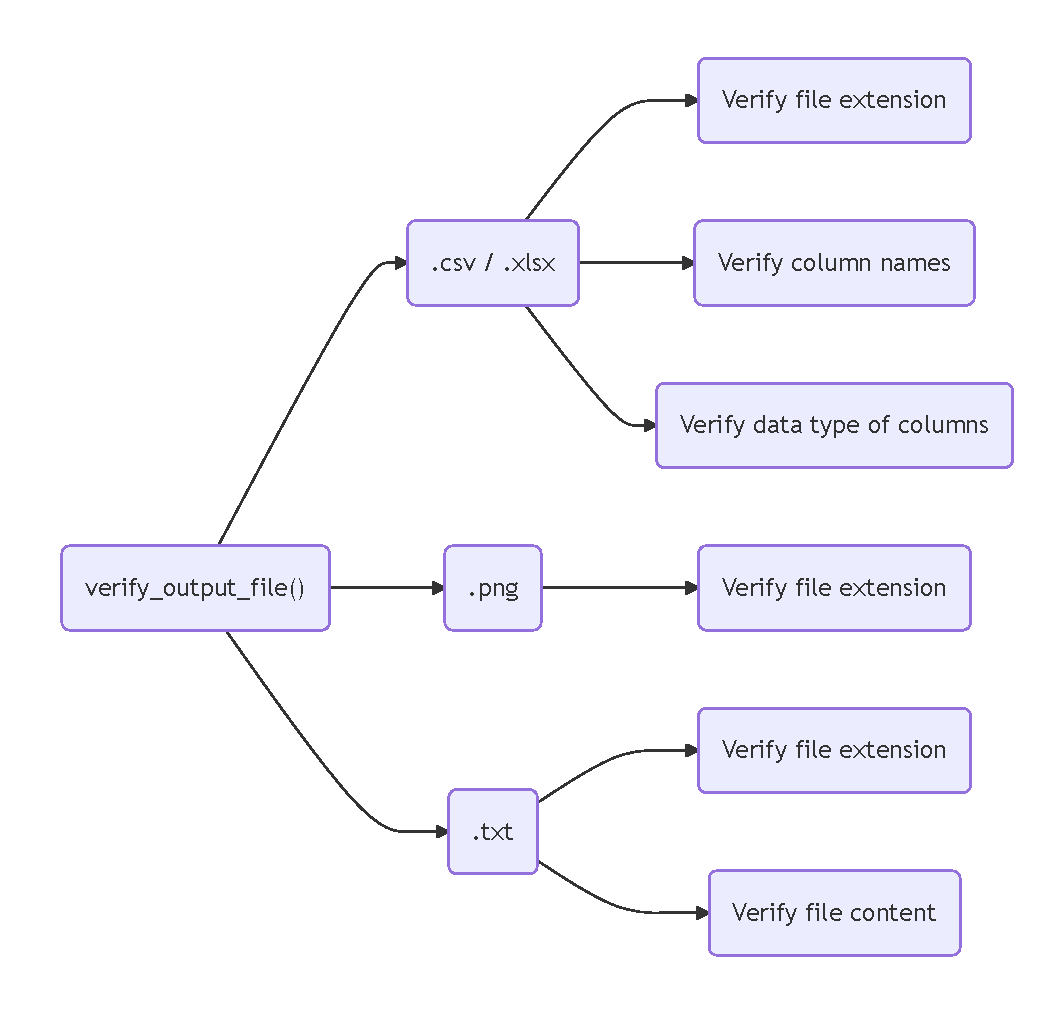
\includegraphics[width=0.8\textwidth]{Images/verify_output_file.pdf}
    \caption{Working of \texttt{verify\_output\_files()} function}
    \label{verify_output_files}
  \end{figure}
  
  To verify the output, we first retrieve the verification data from \texttt{module\_config.json}, which includes properties like column names, file names, 
  formats, and data types. The function iterates through the output folder to check the presence of all output files. Using the Pandas library, it reads 
  \texttt{csv} files to verify column names and data types. If all checks pass, a success message is displayed; otherwise, an error message specifies the issue.

  For non-\texttt{csv} files, the function also verifies the presence and correctness of \texttt{.txt} and \texttt{.png} files. For \texttt{.txt} files, it 
  additionally checks if the file is not empty.
\end{itemize}

\bibliographystyle{plain}
\bibliography{Chapters/references.bib}
\end{spacing}
\end{document}